\documentclass[UTF8]{article}
\usepackage{graphicx}
\usepackage{subfigure}
\usepackage{amsmath}
\usepackage{makecell}
\usepackage[utf8]{inputenc}
\usepackage[space]{ctex} %中文包
\usepackage{listings} %放代码
\usepackage{xcolor} %代码着色宏包
\usepackage{CJK} %显示中文宏包
\usepackage{float}
\usepackage{makecell}
\usepackage{diagbox}
\usepackage{bm}
\usepackage{ulem} 
\usepackage{amssymb}
\usepackage{soul}
\usepackage{color}
\usepackage{geometry}
\usepackage{fancybox} %花里胡哨的盒子
\usepackage{xhfill} %填充包, 可画分割线 https://www.latexstudio.net/archives/8245
\usepackage{multicol} %多栏包
\usepackage{enumerate} %可以方便地自定义枚举标题
\usepackage{multirow} %表格中多行单元格合并
\usepackage{wasysym} %可以使用wasysym里的一堆奇奇怪怪的符号
\usepackage{tikz}
\usepackage{tikZ-timing} % 时序图支持
\usetikzlibrary{arrows,shapes,automata,petri,positioning,calc}
\usetikzlibrary{shadows} % 阴影支持
\usepackage[colorlinks,linkcolor=red]{hyperref} % 超链接支持

\geometry{left = 1.5cm, right = 1.5cm, top=2cm, bottom=2cm}

\definecolor{mygreen}{rgb}{0,0.6,0}
\definecolor{mygray}{rgb}{0.5,0.5,0.5}
\definecolor{mymauve}{rgb}{0.58,0,0.82}
\lstset{
	backgroundcolor=\color{white}, 
	%\tiny < \scriptsize < \footnotesize < \small < \normalsize < \large < \Large < \LARGE < \huge < \Huge
	basicstyle = \footnotesize,       
	breakatwhitespace = false,        
	breaklines = true,                 
	captionpos = b,                    
	commentstyle = \color{mygreen}\bfseries,
	extendedchars = false,
	frame = shadowbox, 
	framerule=0.5pt,
	keepspaces=true,
	keywordstyle=\color{blue}\bfseries, % keyword style
	language = C++,                     % the language of code
	otherkeywords={string}, 
	numbers=left, 
	numbersep=5pt,
	numberstyle=\tiny\color{mygray},
	rulecolor=\color{black},         
	showspaces=false,  
	showstringspaces=false, 
	showtabs=false,    
	stepnumber=1,         
	stringstyle=\color{mymauve},        % string literal style
	tabsize=4,          
	title=\lstname           
}

%\sum\nolimits_{j=1}^{M}   上下标位于求和符号的水平右端,
%\sum\limits_{j=1}^{M}   上下标位于求和符号的上下处,
%\sum_{j=1}^{M}  对上下标位置没有设定,会随公式所处环境自动调整。

%%%%%%%%%%%%%画图包%%%%%%%%%%%%%
\usepackage{tikz}
%%%%%%%%%%%%%好看的矩形%%%%%%%%%%%%%
\tikzset{
  rect1/.style = {
    shape = rectangle,% 指定样式
    minimum height=2cm,% 最小高度
    minimum width=4cm,% 最小宽度
    align = center,% 文字居中
    drop shadow,% 阴影
  }
}
%%%%%%%%%%%%%画图背景包%%%%%%%%%%%%%
\usetikzlibrary{backgrounds}

%%%%%%%%%%%%%在tikz中画一个顶点%%%%%%%%%%%%%
%%%%%%%%%%%%%#1:node名称%%%%%%%%%%%%%
%%%%%%%%%%%%%#2:位置%%%%%%%%%%%%%
%%%%%%%%%%%%%#3:标签%%%%%%%%%%%%%
\newcommand{\newVertex}[3]{\node[circle, draw=black, line width=1pt, scale=0.8] (#1) at #2{#3}}
%%%%%%%%%%%%%在tikz中画一条边%%%%%%%%%%%%%
\newcommand{\newEdge}[2]{\draw [black,very thick](#1)--(#2)}
%%%%%%%%%%%%%在tikz中放一个标签%%%%%%%%%%%%%
%%%%%%%%%%%%%#1:名称%%%%%%%%%%%%%
%%%%%%%%%%%%%#2:位置%%%%%%%%%%%%%
%%%%%%%%%%%%%#3:标签内容%%%%%%%%%%%%%
\newcommand{\newLabel}[3]{\node[line width=1pt] (#1) at #2{#3}}

%%%%%%%%%%%%%强制跳过一行%%%%%%%%%%%%%
\newcommand{\jumpLine} {\hspace*{\fill} \par}
%%%%%%%%%%%%%关键点指令,可用itemise替代%%%%%%%%%%%%%
\newcommand{\average}[1]{\left\langle #1\right\rangle }
%%%%%%%%%%%%%表格内嵌套表格%%%%%%%%%%%%%
\newcommand{\keypoint}[2]{$\bullet$\textbf{#1}\quad#2\par}
%%%%%%%%%%%%%<T>平均值表示%%%%%%%%%%%%%
\newcommand{\tabincell}[2]{\begin{tabular}{@{}#1@{}}#2\end{tabular}}%放在导言区
%%%%%%%%%%%%%大黑点item头%%%%%%%%%%%%%
\newcommand{\itemblt}{\item[$\bullet$]}
%%%%%%%%%%%%%大圈item头%%%%%%%%%%%%%
\newcommand{\itemc}{\item[$\circ$]}
%%%%%%%%%%%%%大星星item头%%%%%%%%%%%%%
\newcommand{\itembs}{\item[$\bigstar$]}
%%%%%%%%%%%%%右▷item头%%%%%%%%%%%%%
\newcommand{\itemrhd}{\item[$\rhd$]}
%%%%%%%%%%%%%定义为%%%%%%%%%%%%%
\newcommand{\defas}{=_{df}}
%%%%%%%%%%%%%蕴含%%%%%%%%%%%%%
\newcommand{\imp}{\rightarrow}

%%%%%%%%%%%%%双线分割线%%%%%%%%%%%%%
\newcommand*{\doublerule}{\hrule width \hsize height 1pt \kern 0.5mm \hrule width \hsize height 2pt}
%%%%%%%%%%%%%双线中间可加东西的分割线%%%%%%%%%%%%%
\newcommand\doublerulefill{\leavevmode\leaders\vbox{\hrule width .1pt\kern1pt\hrule}\hfill\kern0pt }
%%%%%%%%%%%%%左大括号%%%%%%%%%%%%%
\newcommand{\leftbig}[1]{\left\{\begin{array}{l}#1\end{array}\right.}
%%%%%%%%%%%%%矩阵%%%%%%%%%%%%%
\newcommand{\mat}[2]{\left[\begin{array}{#1}#2\end{array}\right]}
%%%%%%%%%%%%%可换行圆角文本框%%%%%%%%%%%%%

\newcommand{\ovalboxn}[1]{\ovalbox{\tabincell{l}{#1}}}
%%%%%%%%%%%%%设置section的counter, 使从0开始%%%%%%%%%%%%%

\title{编译原理与技术 H2}
\date{}
\author{PB18111697 王章瀚}

\begin{document}
\maketitle
\section{教材2.7(d)}
\ovalboxn{为下列正规式手工构造NFA和DFA, 再用算法将NFA变换成DFA并构造最简的DFA.\\$(a|b)^*abb(a|b)^*$}\\
\begin{enumerate}
\item 手工构造NFA, 如下图所示\\
	\begin{center}
	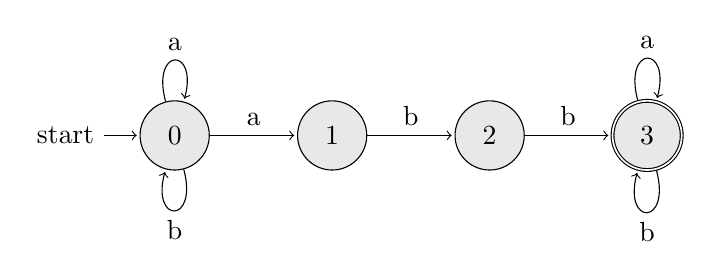
\begin{tikzpicture}[shorten >=1pt,node distance=2cm,auto]
	\tikzstyle{every state}=[fill={rgb:black,1;white,10}]
	
	\node[state,initial](0){0};
	\node[state](1)[right of=0]{1};
	\node[state](2)[right of=1]{2};
	\node[state, accepting](3)[right of=2]{3};
	
	\path[->] (0) edge[loop above] node{a} ();
	\path[->] (0) edge[loop below] node{b} ();
	\path[->] (0) edge node{a} (1);
	\path[->] (1) edge node{b} (2);
	\path[->] (2) edge node{b} (3);
	\path[->] (3) edge[loop above] node{a} ();
	\path[->] (3) edge[loop below] node{b} ();
	\end{tikzpicture}
	\end{center}
\item 手工构造DFA, 如下图所示\\
	\begin{center}
	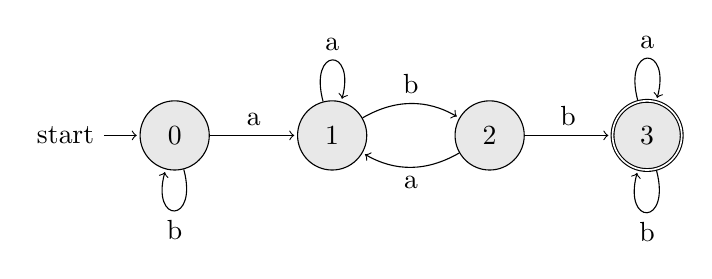
\begin{tikzpicture}[shorten >=1pt,node distance=2cm,auto]
	\tikzstyle{every state}=[fill={rgb:black,1;white,10}]
	
	\node[state,initial](0){0};
	\node[state](1)[right of=0]{1};
	\node[state](2)[right of=1]{2};
	\node[state, accepting](3)[right of=2]{3};
	
	\path[->] (0) edge[loop below] node{b} ();
	\path[->] (0) edge node{a} (1);
	\path[->] (1) edge[loop above] node{a} (1);
	\path[->] (1) edge[bend left] node{b} (2);
	\path[->] (2) edge[bend left] node{a} (1);
	\path[->] (2) edge node{b} (3);
	\path[->] (3) edge[loop above] node{a} ();
	\path[->] (3) edge[loop below] node{b} ();
	\end{tikzpicture}
	\end{center}
\item 将NFA变换成DFA, 即使用子集构造法.\\
	\begin{minipage}[H]{0.3\linewidth}
	\begin{tabular}{|c|c|c|}
	\hline
	\multirow{2}{*}{状态} & \multicolumn{2}{c|}{输入符号} \\
						  \cline{2-3}
						  & a & b \\
    \hline
	A & B & A \\
	\hline
	B & B & C \\
	\hline
	C & B & D \\
	\hline
	D & E & D \\
	\hline
	E & E & F \\
	\hline
	F & E & D\\
	\hline
	\end{tabular}\\
	\end{minipage}
	\begin{minipage}[H]{0.3\linewidth}
	\jumpLine
	其中, \begin{itemize}
	\item 状态A=\{0\}
	\item 状态B=\{0, 1\}
	\item 状态C=\{0, 2\}
	\item 状态D=\{0, 3\}
	\item 状态E=\{0, 1, 3\}
	\item 状态F=\{0, 2, 3\}
	\end{itemize}
	\end{minipage}
	
	\begin{center}
	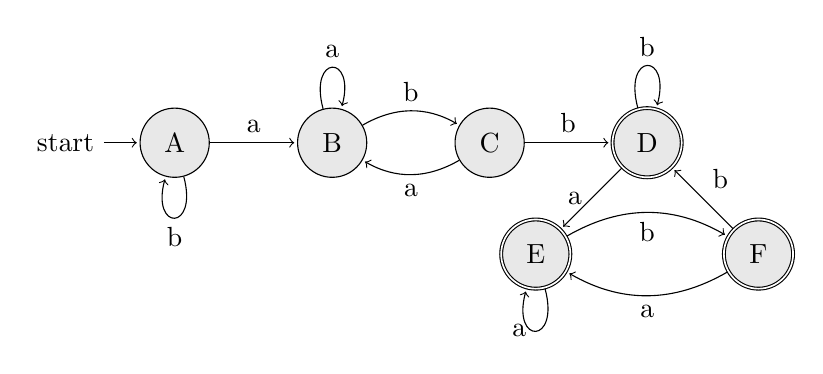
\begin{tikzpicture}[shorten >=1pt,node distance=2cm,auto]
	\tikzstyle{every state}=[fill={rgb:black,1;white,10}]
	\node[state, initial](A){A};
	\node[state](B)[right of=A]{B};
	\node[state](C)[right of=B]{C};
	\node[state, accepting](D)[right of=C]{D};
	\node[state, accepting](E)[below left of=D]{E};
	\node[state, accepting](F)[below right of=D]{F};
	
	\path[->] (A) edge node{a} (B);
	\path[->] (A) edge[loop below] node{b} ();
	\path[->] (B) edge[loop above] node{a} ();
	\path[->] (B) edge[bend left] node{b} (C);
	\path[->] (C) edge[bend left] node{a} (B);
	\path[->] (C) edge node{b} (D);
	\path[->] (D) edge node[left]{a} (E);
	\path[->] (D) edge[loop above] node{b} ();
	\path[->] (E) edge[loop below] node[left]{a} (E);
	\path[->] (E) edge[bend left] node[below]{b} (F);
	\path[->] (F) edge[bend left] node{a} (E);
	\path[->] (F) edge node[above right]{b} (D);
	\end{tikzpicture}
	\end{center}
\item 构造最简的DFA\\
	前面构造的DFA对应转换函数是全函数, 因此不必引入死状态.
	\begin{enumerate}[(1)]
	\item 按是否含接受状态划分为两个集合$\{A, B, C\}$和$\{D,E,F\}$. 这时有
	$$\begin{array}{l}
	move(\{A, B, C\},a)=\{B\}\in\{A,B,C\}\\
	move\{A,B,C\},b)=\{A,C,D\}\rightarrow\mbox{C经b得D}\\
	move(\{D,E,F\},a)=\{E\}\in\{D,E,F\}\\
	move(\{D,E,F\},b)=\{D,F\}\in\{D,E,F\}\\
	\end{array}$$
	因此得到新划分: $\{A,B\}, \{C\},\{D,E,F\}$
	\item 再作第二次划分. 只有$\{A,B\}$和$\{D,E,F\}$有划分的可能 
	$$\begin{array}{l}
	move(\{A,B\},a)=\{B\}\in\{A,B\}\\
	move(\{A,B\},b)=\{A,C\}\rightarrow\mbox{B经b得C}\\
	move(\{D,E,F\},a)=\{E\}\in\{D,E,F\}\\
	move(\{D,E,F\},b)=\{D,F\}\in\{D,E,F\}\\
	\end{array}$$
	因此得到新划分: $\{A\}, \{B\}, \{C\},\{D,E,F\}$
	\end{enumerate}
	因此, 可以构造出最简的DFA(将$\{D,E,F\}$看作D):
	\begin{center}
	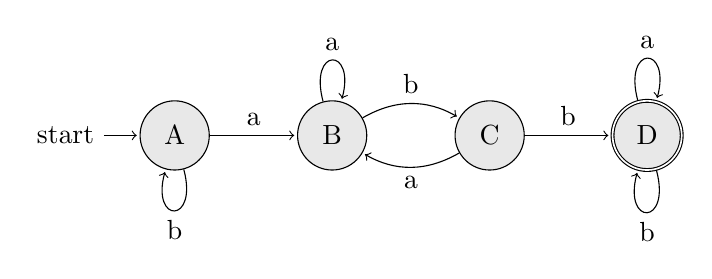
\begin{tikzpicture}[shorten >=1pt,node distance=2cm,auto]
	\tikzstyle{every state}=[fill={rgb:black,1;white,10}]
	\node[state, initial](A){A};
	\node[state](B)[right of=A]{B};
	\node[state](C)[right of=B]{C};
	\node[state, accepting](D)[right of=C]{D};
	
	\path[->] (A) edge node{a} (B);
	\path[->] (A) edge[loop below] node{b} ();
	\path[->] (B) edge[loop above] node{a} ();
	\path[->] (B) edge[bend left] node{b} (C);
	\path[->] (C) edge[bend left] node{a} (B);
	\path[->] (C) edge node{b} (D);
	\path[->] (D) edge[loop above] node{a} ();
	\path[->] (D) edge[loop below] node{b} ();
	\end{tikzpicture}
	\end{center}

\end{enumerate}

\end{document}


